\chapter{TrackML}
\label{chapter:TrackML}

\section{TrackML Challenge}

To bring expertise for particle tracking for Run-3 to CERN from the computer science and machine learning communities, several LHC experiments have worked together to invite machine learning teams from outside CERN to compete in the 2018 Kaggle challenge called the TrackML Particle Tracking Challenge~\cite{TrackML}~\cite{TrackMLPPTBefore}~\cite{TrackMLPPTAfter}~\cite{TrackMLPPTAfter2} and a follow-up challenge in 2019~\cite{TrackML2}.

\ \\The candidates were offered a dataset of simulated charged particles in a general-purpose detector, representative of ATLAS and CMS at CERN. The simulation contains both the true and reconstructed position of the track hits, allowing for a labelled dataset on which learning can be performed. The dataset was obtained using a common tracking software framework at CERN called ACTS~\cite{ACTS}~\cite{ACTSPPT}. Events of top quark production (\ttbar~events) were simulated at $\mu=200$, leading to about 10 thousand tracks per event. \ttbar~events are known to produce many particles and consequently also many tracks. 

\ \\Tracks are reconstructed in the inner detector, which is simulated to be formed of three types of silicon detectors, to be representative of both the ATLAS and CMS at the planned High Luminosity LHC (HL-LHC). As illustrated in Figure~\ref{fig:ThreeSiDetectors}, the three silicon detectors are the pixels, short strips and long strips, in order of increasing radius. 

\begin{figure}[htb]
\centering
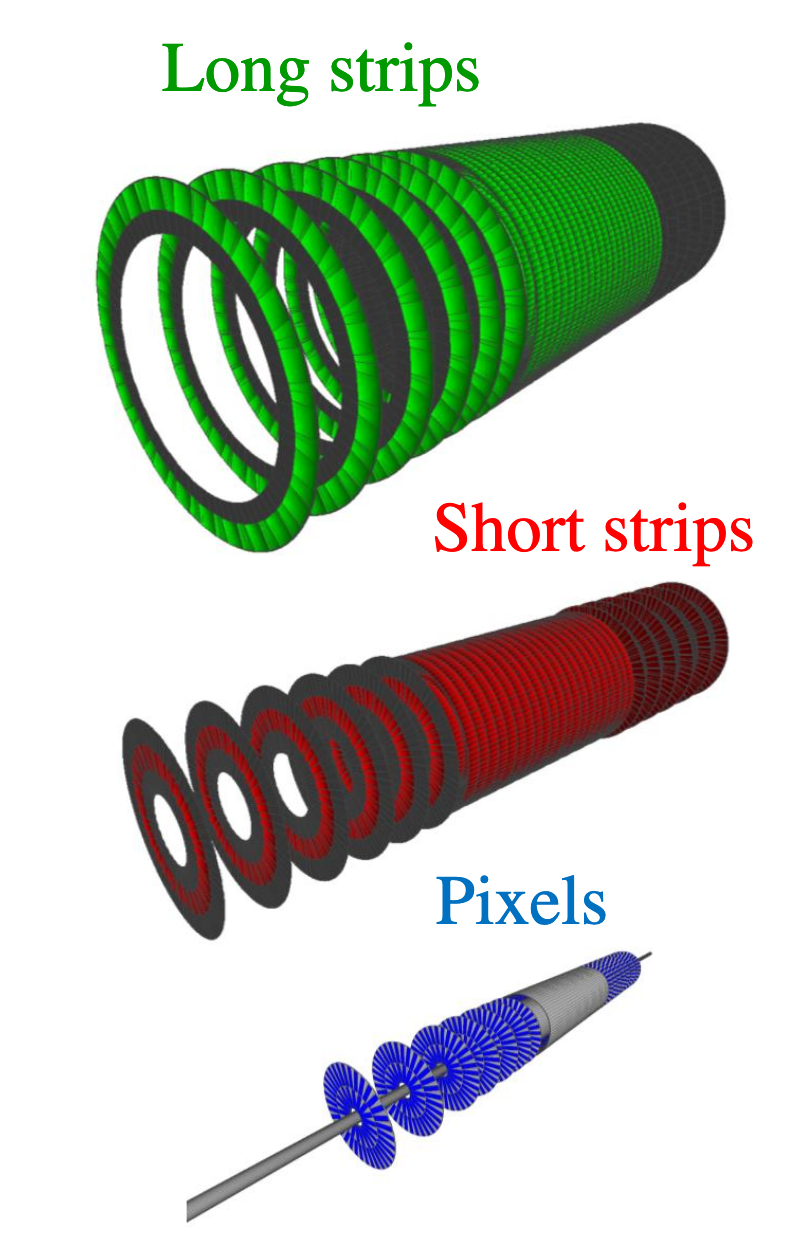
\includegraphics[width=0.45\textwidth]{./plots/ThreeSiDetectors.png}
\caption{Tracks are reconstructed in the inner detector, which is simulated to be formed of three types of silicon detectors. From beam pipe outwards the pixels, short strips and long strips~\cite{TrackMLPPTBefore}~\cite{TrackMLPaperAccuracyPhase}.}
\label{fig:ThreeSiDetectors}
\end{figure}

\ \\The coordinate system is right-handed and cartesian. The z-axis points along the beam axis (longitudinal axis). The x-y plane is the transverse plane. The azimuthal angle $\phi$ with values within $[0, 2\pi)$ is the angle in the transverse plane to the x-axis. The polar angle $\theta$ with values within $[0, \pi]$ is the angle to the z-axis. In particle physics, instead of the angle $\theta$ often the pseudo-rapidity $\eta$ is used, where $\eta = -\ln \tan (\theta/2)$.

\ \\In this coordinate system, the three silicon detectors are presented in the longitudinal plane in the left side of Figure~\ref{fig:DetectorGeometry}. The horizontal lines represent the barrel, and the vertical lines represent the two end-caps of the detector. The pixel detector is shown in the transverse plane in the right side of~\ref{fig:DetectorGeometry}. 

\begin{figure}[hbt]
\centering
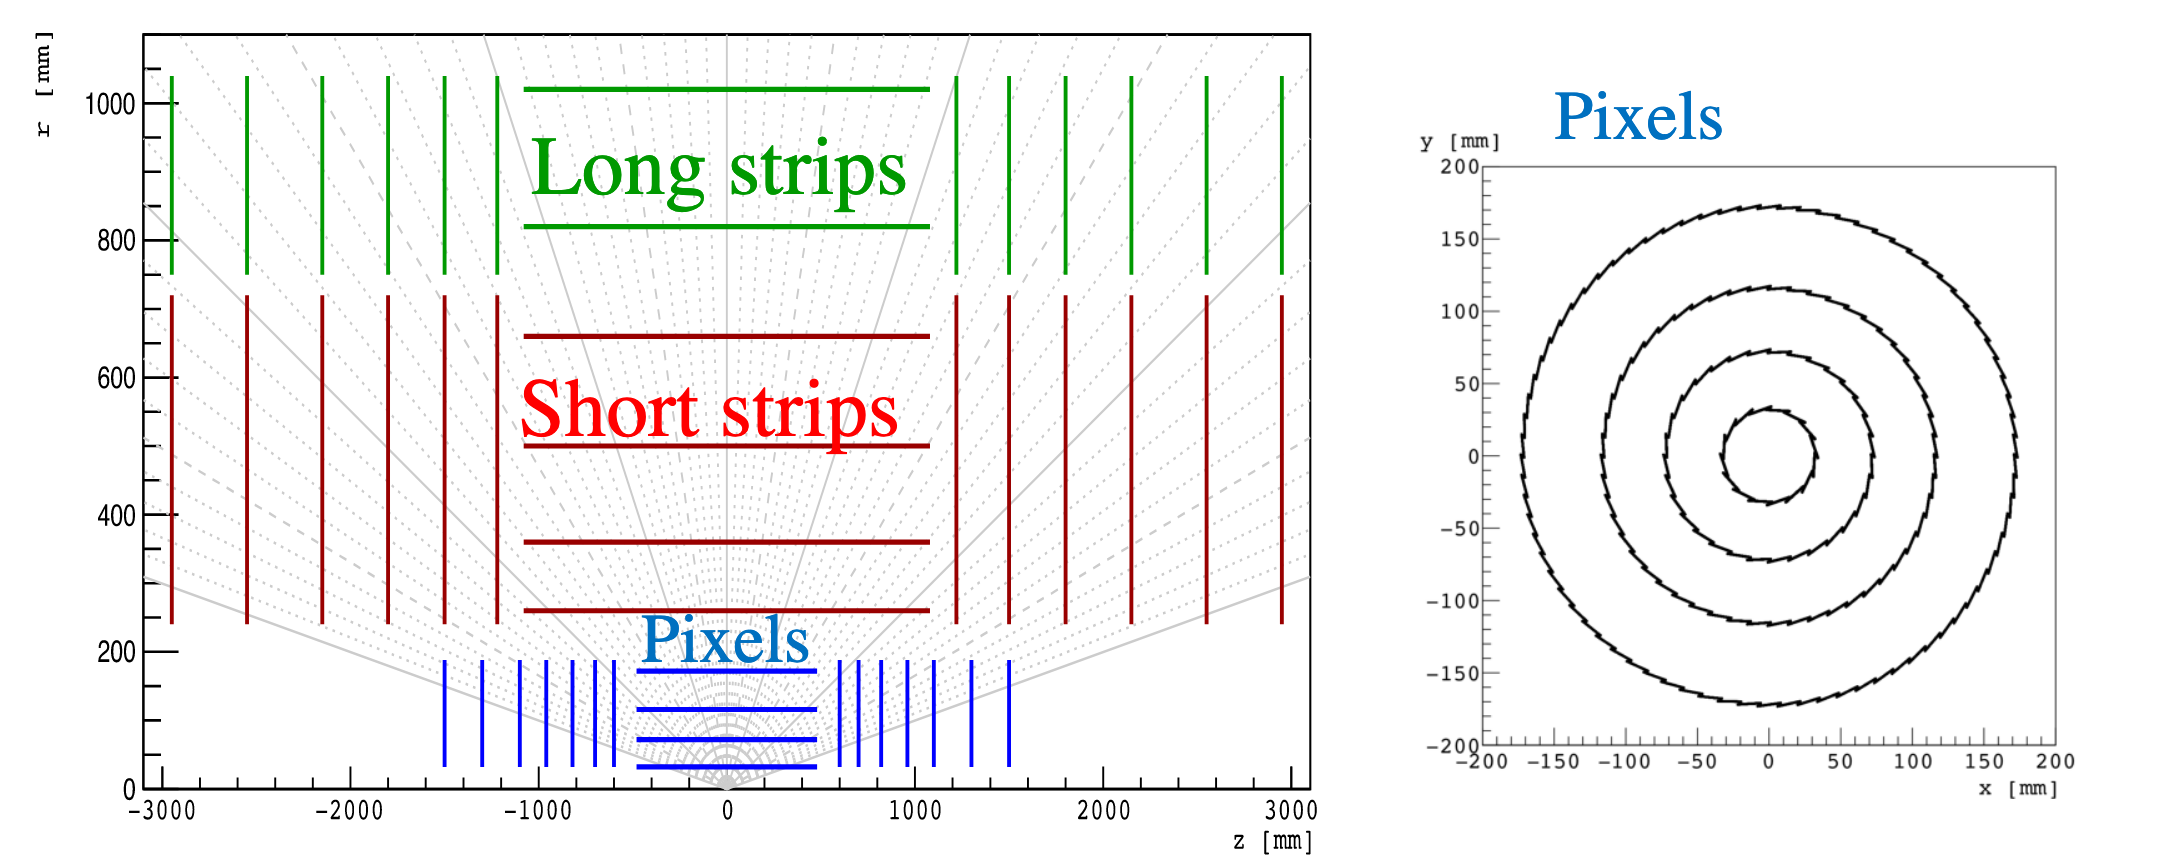
\includegraphics[width=0.9\textwidth]{./plots/DetectorGeometry.png}
\caption{The three detectors are organized in volumes, layers and modules~\cite{TrackMLPPTBefore}~\cite{TrackMLPaperAccuracyPhase}.}
\label{fig:DetectorGeometry}
\end{figure}

\section{Dataset}

Ten thousand events were simulated with collisions in the centre of the detector, leading to about 0.1 billion tracks. Each track has about 10 hits, or 3D points, in the simulated detector, leading to a total of 1 billion points, and about 100 GBytes of data~\cite{TrackMLPPTAfter2}. The dataset from TrackML is described in detail in~\cite{TrackMLPaperAccuracyPhase}~\cite{TrackMLPaper}~\cite{TrackMLPaperHAL}. A subset of 100 events of the TrackML dataset is used in this study.

\ \\The detector volumes for barrel and end-caps are divided into unique \volumeID. Each volume is divided into layers described by \layerID, which for technical reasons have only even values. Each layer is divided into modules identified by \moduleID. For each event, four files are provided~\cite{TrackMLPaper}, as described below.

\ \\The \emph{hit} file contains the reconstructed hit information: \hitID, the numerical identifier of the hit within the event, the measured coordinates $x$, $y$, $z$ of the hit in mm, the \volumeID, the \layerID, and the \moduleID.

\ \\The \emph{truth} file contains the generated (also called truth) hit information: the \hitID, the \particleID~of the particle that generated this hit, the truth coordinates $tx$, $ty$, $tz$ in mm, and the truth momenta $tpx$, $tpy$, $tpz$. 

\ \\The \emph{particles} file contains for each \particleID~the particle type, its velocities and momenta, the electric charge and the number of hits.

\ \\The \emph{cells} file contains for each \hitID~the cell that recorded the hit. A cell is the smallest unit in a particle detector. A cell is identified uniquely by two channel numbers, similarly to two coordinates of a pixel in an image. 

\ \\In this thesis only the \emph{hit} and \emph{truth} files of 100 events simulated with $\mu=200$ are studied. They are read in as data frames, and concatenated by columns. As a result, for each \hitID~one knows the reconstructed coordinates, the truth coordinates, truth momenta and to what \particleID~it belongs to. 

\section{Simulated Truth Particles and Reconstructed Hits}

One random event with index 99 is studied. Its behaviour is however representative for all events. A typical event produces about 10 thousand simulated particles, with a distribution of the number of hits per particle illustrated in Figure~\ref{fig:TruthParticleNbHits}, with a mean of 10.8 and a standard deviation (rms) of 3.3.

\begin{figure}[htb]
\centering
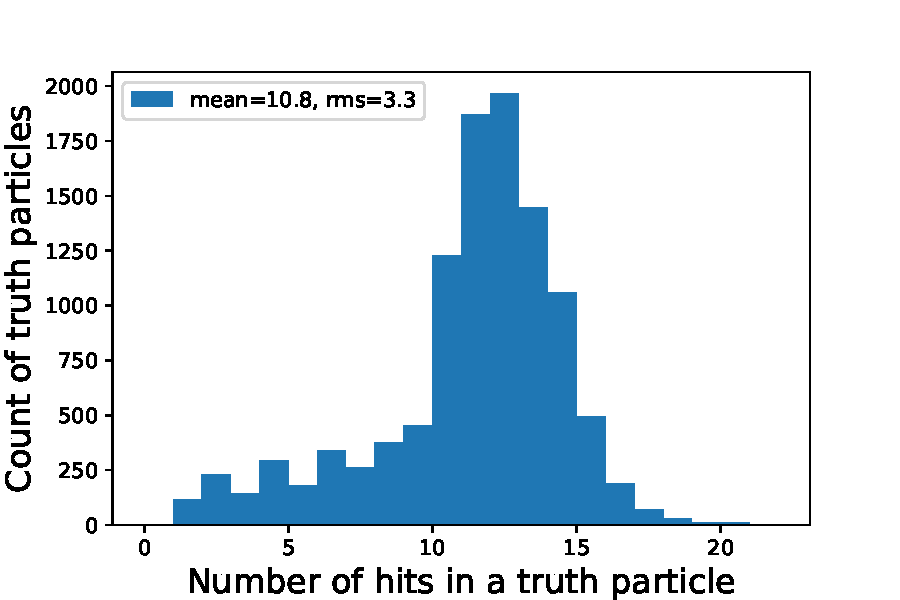
\includegraphics[width=0.45\textwidth]{plots/DataExploration_histo_counterTruthParticles_vs_nbHitsInTruthParticle.pdf}
\caption{Distribution of the number of hits in truth particles in event 99}
\label{fig:TruthParticleNbHits}
\end{figure}

%\ \\All collisions are simulated in the center of the detector, and all particles emerge from very close to the center of the detector. There are no particles travelling far away from the center of the detector, which is represented physically by no cosmic ray particles being considered in the sample. To double check this, for each truth particle of event 99, the $r$ and $z$ coordinates of all hist belonging to the particle are fit to a straight line of equation $y=a_0+a_1x$. $a_0$ is the $r$ value at $z=0$, while $a_1$ is the tangent of the slope angle. $z_0 = -a_0/a_1$ is the $z$ coordinate at zero radius $r$. Both $a_0$ and $z_0$ should be very close to zero for particles simulated in the center of the detector, and have large values for cosmic particles. Their distribution, illustrated in Figure~\ref{fig:TruthParticleFit} confirm that indeed there are no cosmic particle and all particles are simulated in the center of the detector. Furthermore, the angle of the particles peaks at -90 and 90 degrees, meaning that most particles are emitted in the transverse plane. Indeed, it is expected from a so called hard-scatter collision, like the \ttbar~events simulated for TrackML.

%\begin{figure}[!htb]
%\centering
%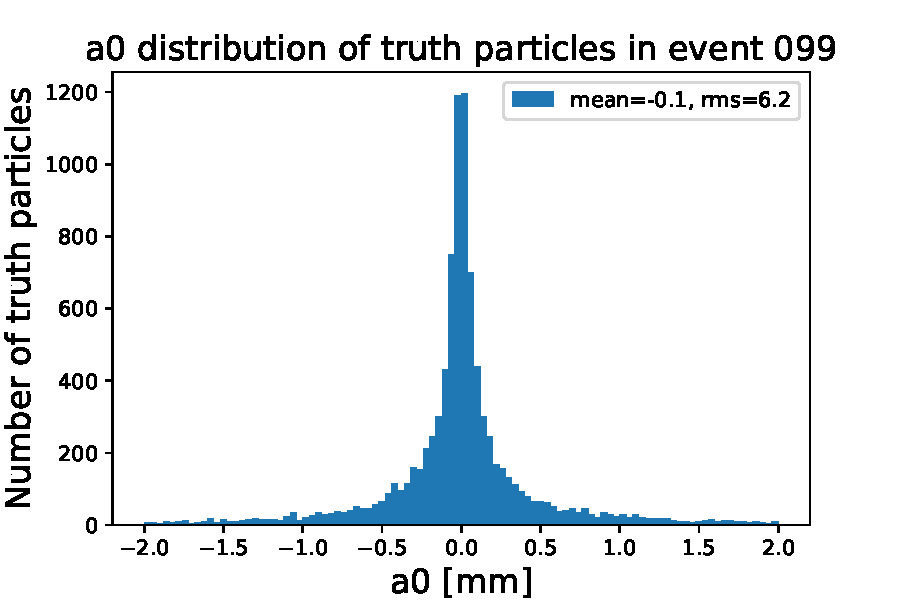
\includegraphics[width=0.45\textwidth]{plots/DataExploration_a0.pdf}
%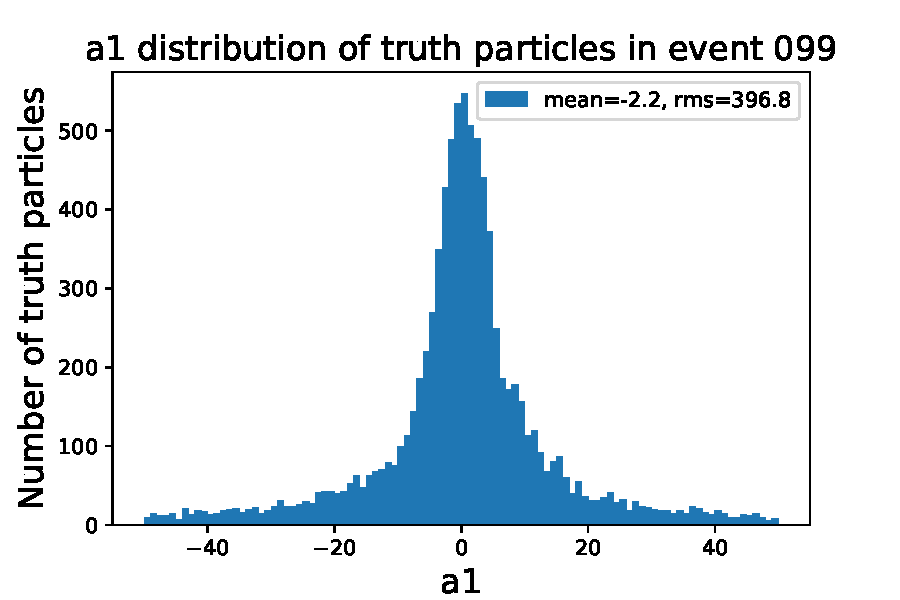
\includegraphics[width=0.45\textwidth]{plots/DataExploration_a1.pdf}\\
%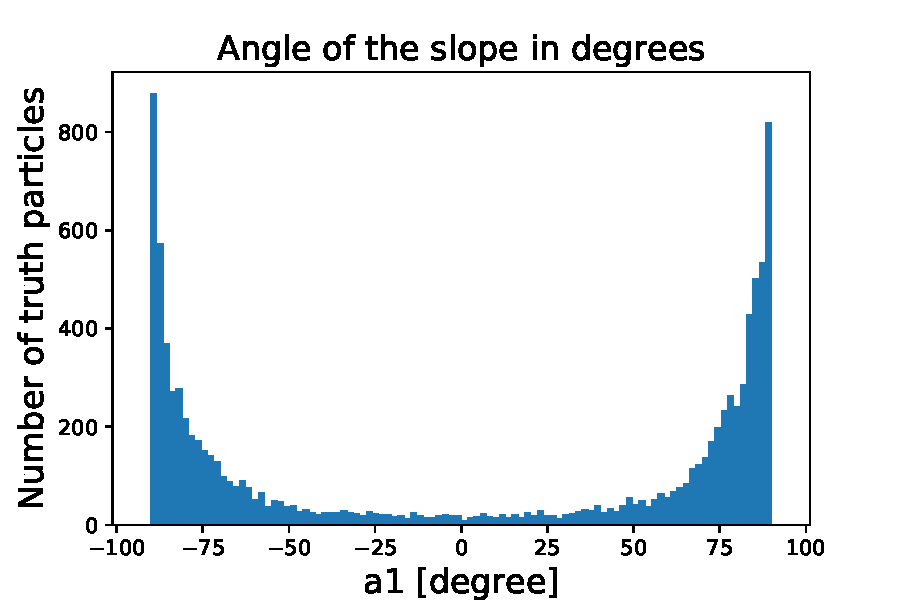
\includegraphics[width=0.45\textwidth]{plots/DataExploration_a1_degree.pdf}
%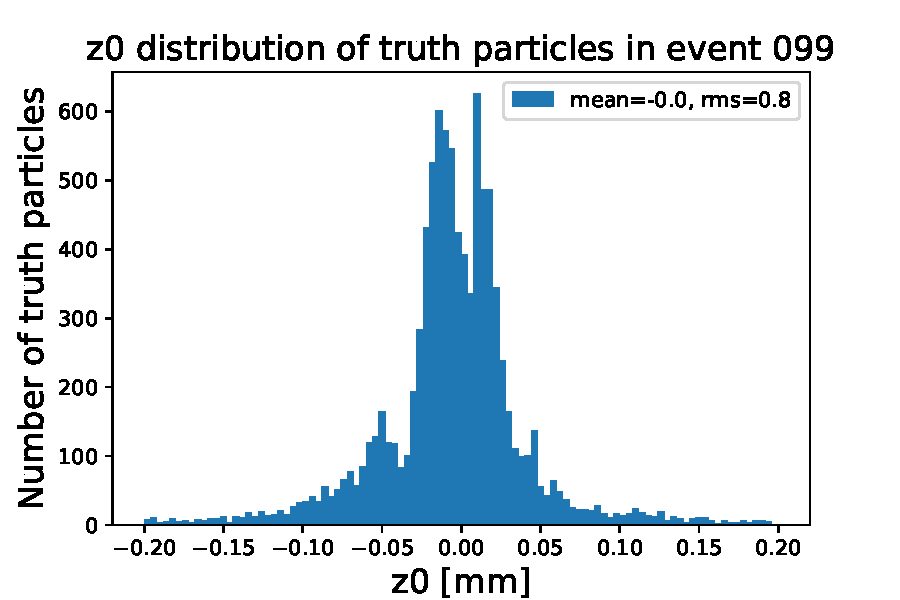
\includegraphics[width=0.45\textwidth]{plots/DataExploration_z0.pdf}
%\caption{$a_0$ [mm], $a_1$,  $a_1$ [degree], $z_0$ [mm] distributions for all truth particles in event 99.}
%\label{fig:TruthParticleFit}
%\end{figure}

\ \\Particles produced in the collisions in the centre of the detector travel in all possible directions. Four tracks made of hits for truth particles, going to both left and right, at an angle closer to the transverse plane, or to the z-axis, are shown in Figure~\ref{fig:TruthParticleTracks}. The images confirm that the hits for each particle are grouped along a line. The $z$ and radius $r$ coordinates are fit to a line of equation ($r = a_0 + a_1 \cdot x$). $a_0$ represents the intercept, or the radius when $z=0$, at the centre of the detector. The values of $a_0$ that are close to zero are consistent with the particles being emitted from the centre of the detector. $a_1$ represents the slope of the line. The fact that $a_0$ have different values, both positive and negative, show that particles are emitted in all directions. $z_0$ represents the $z$ position when the radius $r=0$, meaning when the particle line intersects the z-axis. The fact that the $z_0$ values are close to zero is consistent again with the particles being emitted in the centre of the detector.

\begin{figure}[htb]
\centering
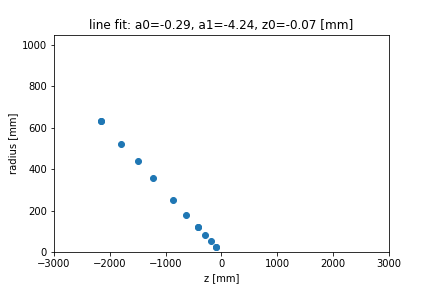
\includegraphics[width=0.35\textwidth]{plots/particle_553945090628780032_r_vs_z.png}
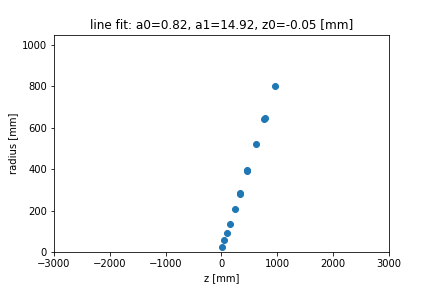
\includegraphics[width=0.35\textwidth]{plots/particle_540433329673994240_r_vs_z.png}\\
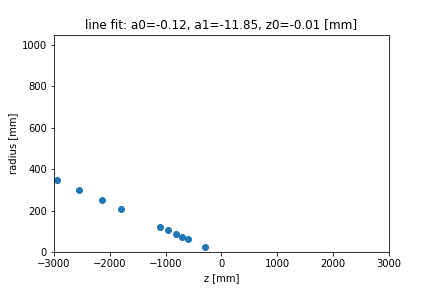
\includegraphics[width=0.35\textwidth]{plots/particle_94575729613733888_r_vs_z.png}
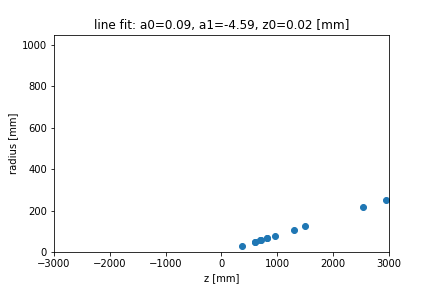
\includegraphics[width=0.35\textwidth]{plots/particle_99081047228022784_r_vs_z.png}
\caption{Four truth particle tracks from event 99 travelling in all possible directions shown in the longitudinal r-z plane. A straight line of equation $r = a_0 + a_1 \cdot x$ is fitted to the points. $a_0$ is the intercept and $a_1$ is the slope. $z_0$ is the $z$ coordinate when the radius $r=0$.}
\label{fig:TruthParticleTracks}
\end{figure}

%\section{Reconstructed hits}
\ \\The reconstructed hit coordinates $x$, $y$, $z$ are very close to the corresponding truth values, as illustrated in Figure~\ref{fig:ReconstructedToTruthHits}. The reconstructed scale and resolution values are therefore good. 

\begin{figure}[htb]
\centering
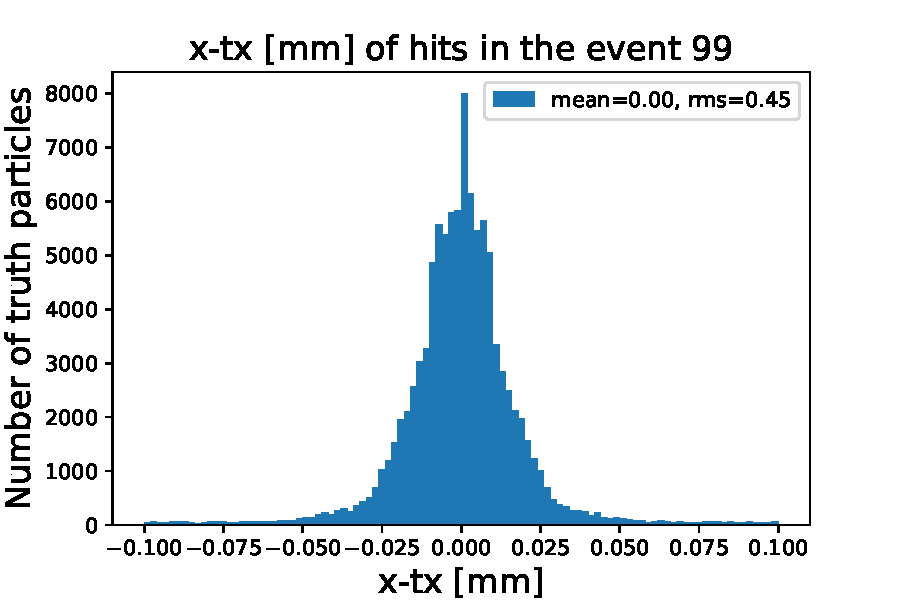
\includegraphics[width=0.32\textwidth]{plots/DataExploration_x_tx.pdf}
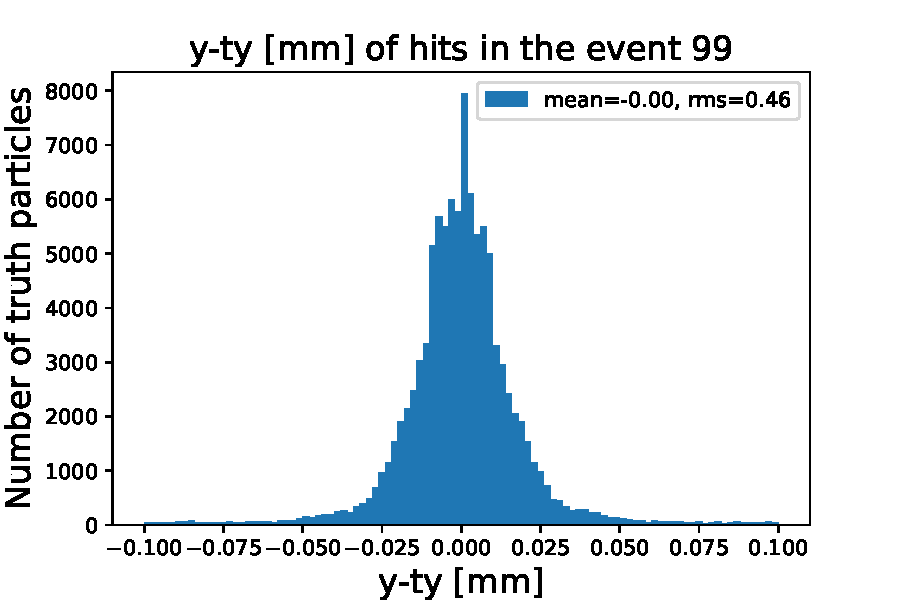
\includegraphics[width=0.32\textwidth]{plots/DataExploration_y_ty.pdf}
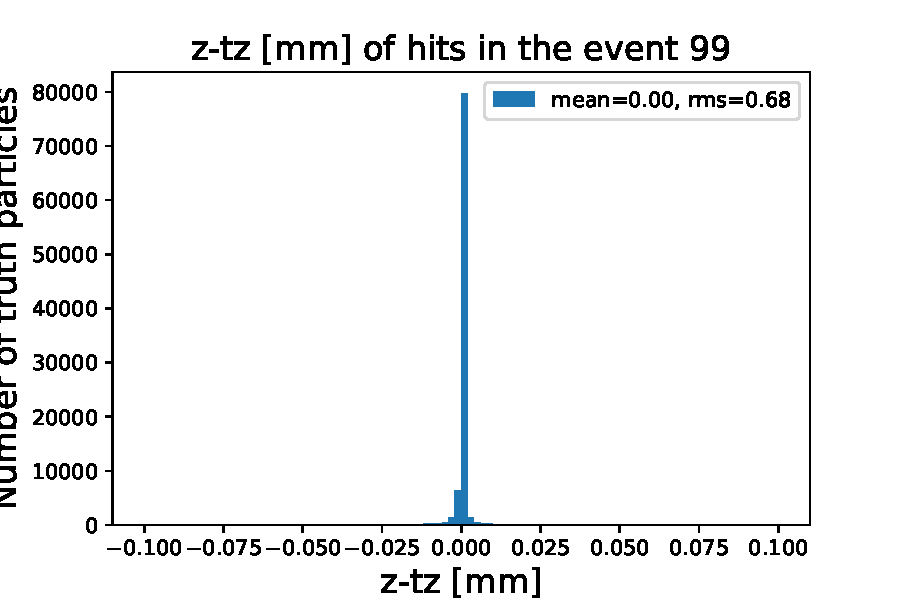
\includegraphics[width=0.32\textwidth]{plots/DataExploration_z_tz.pdf}
\caption{Distributions of reconstructed values minus truth values for $x$, $y$, $z$ in mm for all truth particles in event 99}
\label{fig:ReconstructedToTruthHits}
\end{figure}

\ \\Their coordinates, plus the $r$ coordinate, are illustrated in Figure~\ref{fig:ReconstructedHits}. 

\begin{figure}[htb]
\centering
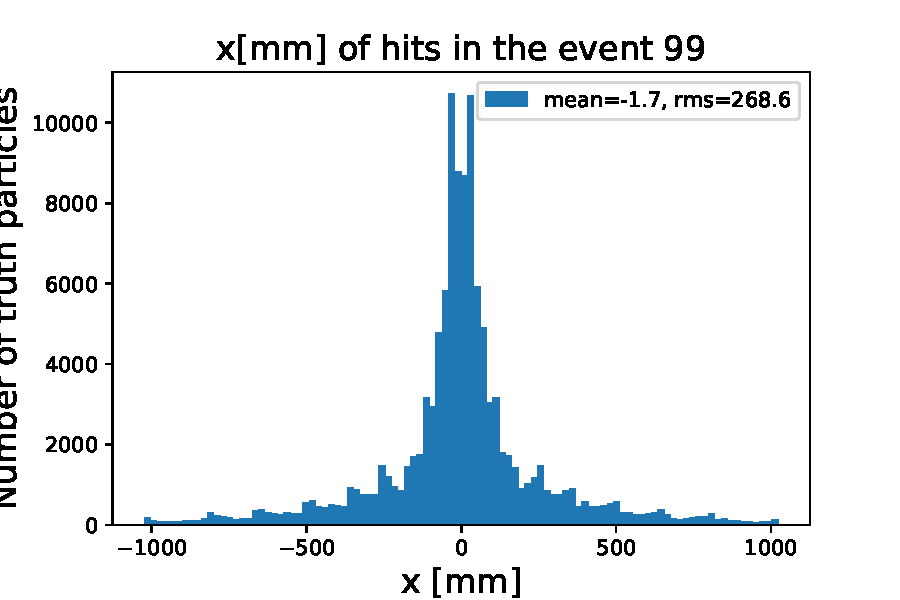
\includegraphics[width=0.35\textwidth]{plots/DataExploration_x.pdf}
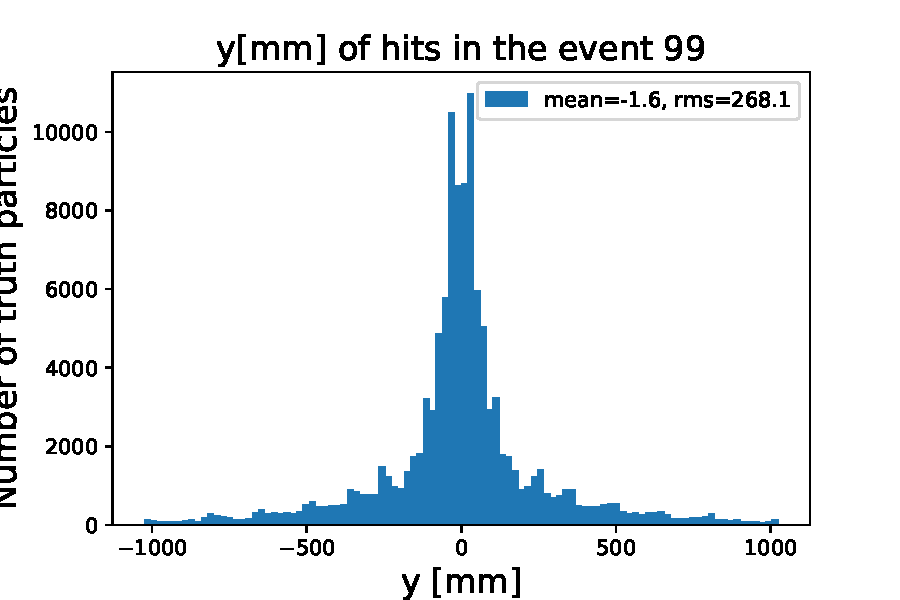
\includegraphics[width=0.35\textwidth]{plots/DataExploration_y.pdf}\\
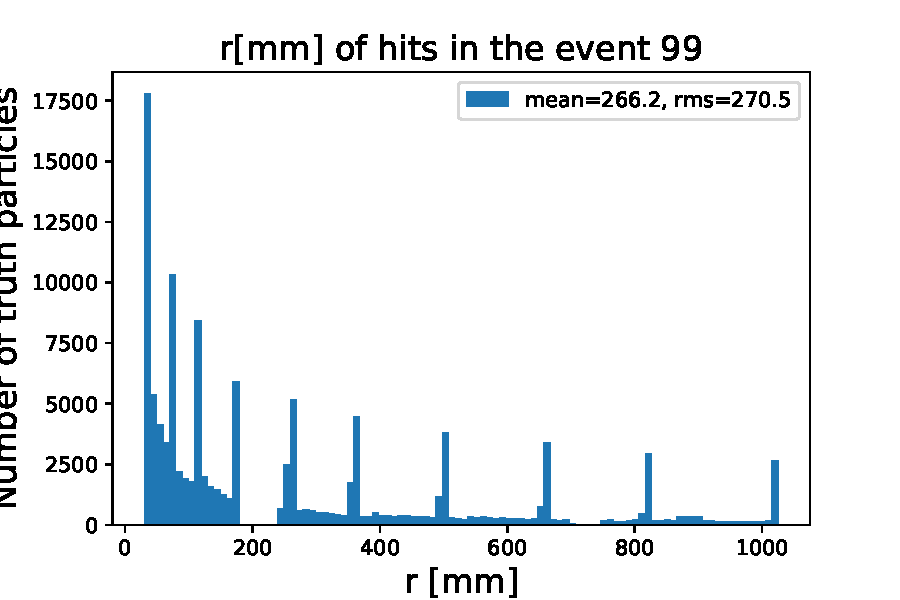
\includegraphics[width=0.35\textwidth]{plots/DataExploration_r.pdf}
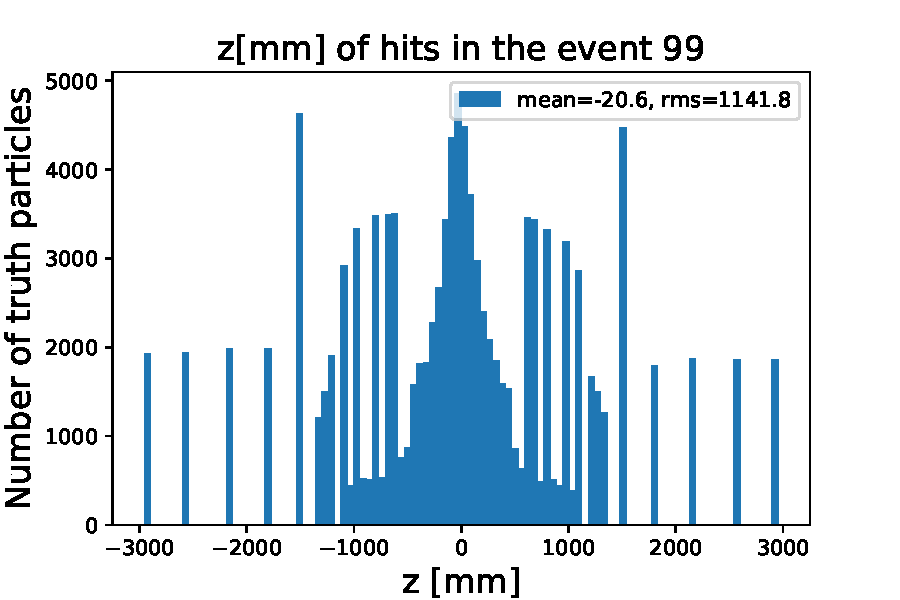
\includegraphics[width=0.35\textwidth]{plots/DataExploration_z.pdf}
\caption{$x$, $y$, $r$, $z$ distributions in mm for all truth particles in event 99}
\label{fig:ReconstructedHits}
\end{figure}

\section{Detector Components}

The grouping of hits inside the detector is used later in this study to evaluate the performance of the model in each detector sub-volume called \volumeID. The detector is formed by a central barrel and two end-caps. There are three layers of volumes from the beam outwards. The volumes from the barrel (end-caps) have the modules alligned horizontally (vertically). Most hits are detected in the volumes of the inner layer, and in those of the barrel. This is consistent with hard-scatter collisions emitted mostly at high $\pt$, so close to the transverse plane. The \volumeID~numbers are visualised in Figure~\ref{fig:DetectorVolumeIDLayerID}, along with the percentage of the hits in each \volumeID, as measured in 100 simulated event in this study. Also Figure~\ref{fig:DetectorHits} illustrates the clustering of hits by \volumeID, \layerID, and \moduleID. The 2D scatter plots between the \volumeID~and the \moduleID~on one side and the $r$ and $z$ on the other side are illustrated in Figure~\ref{fig:ScatterPlotHits}. 

\begin{figure}[!hbt]
\centering
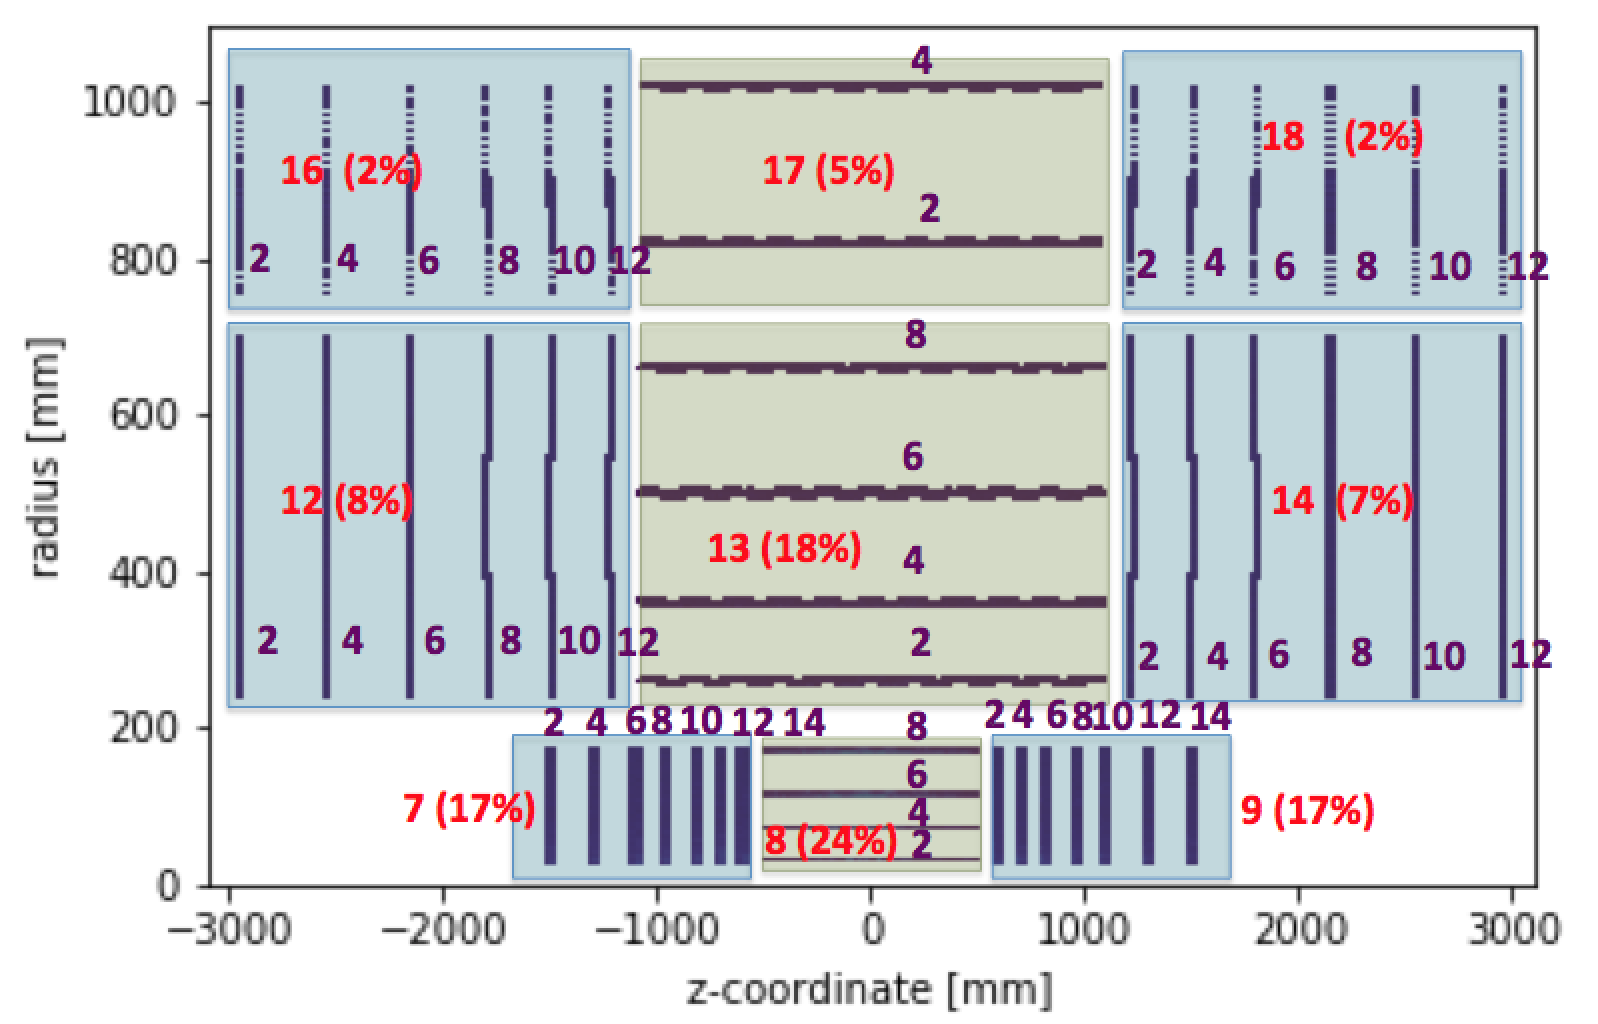
\includegraphics[width=0.9\textwidth]{./plots/DetectorVolumeIDLayerID.png}
\caption{Percentage of hits from 100 events in each volume ID and layer ID}
\label{fig:DetectorVolumeIDLayerID}
\end{figure}

\begin{figure}[!htb]
\centering
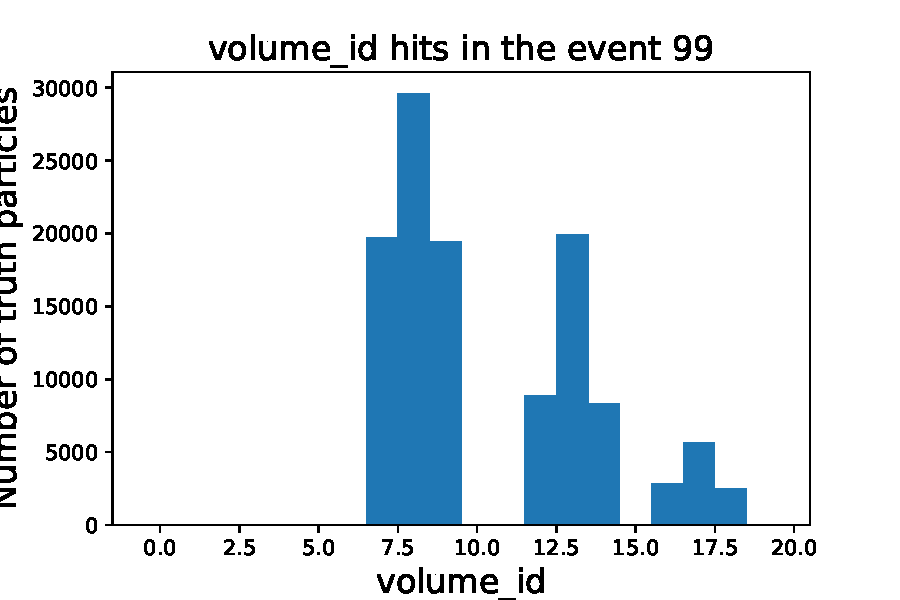
\includegraphics[width=0.32\textwidth]{plots/DataExploration_volume_id.pdf}
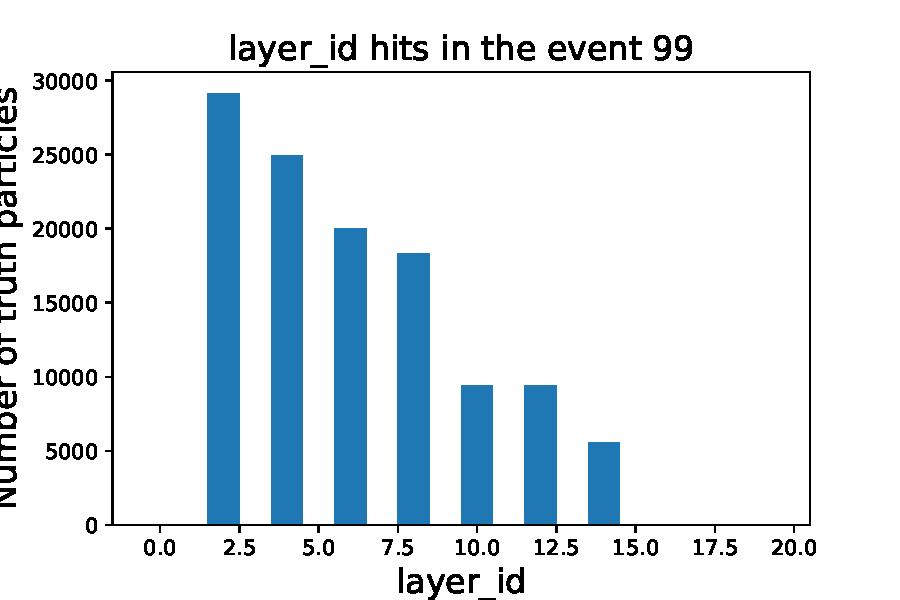
\includegraphics[width=0.32\textwidth]{plots/DataExploration_layer_id.pdf}
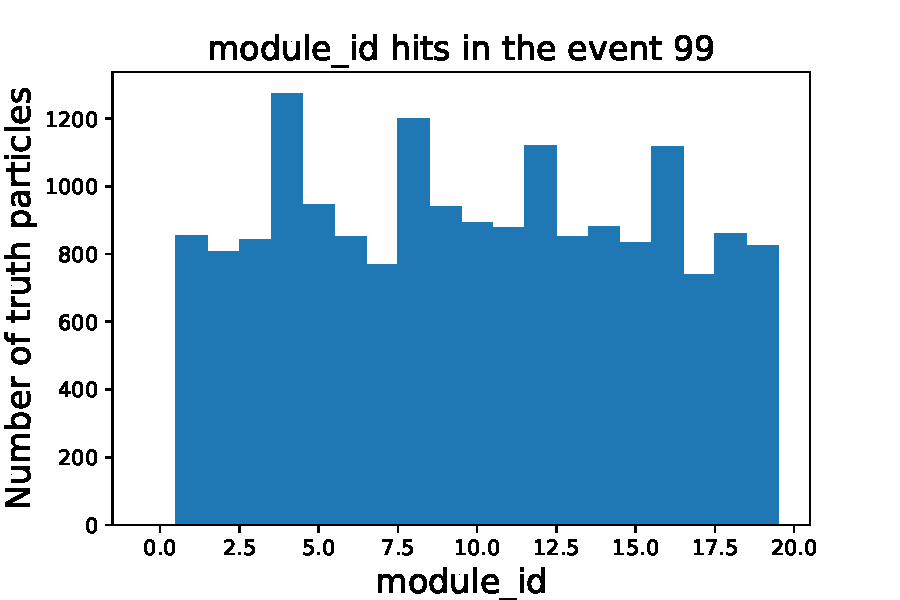
\includegraphics[width=0.32\textwidth]{plots/DataExploration_module_id.pdf}
\caption{Distributions of reconstructed hits in the various volume ID, layer ID and module ID, for all truth particles in event 99}
\label{fig:DetectorHits}
\end{figure}

\begin{figure}[!htb]
\centering
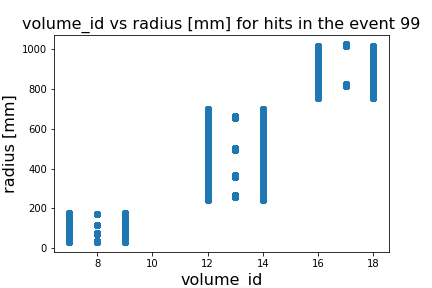
\includegraphics[width=0.35\textwidth]{plots/DataExploration_volume_id_r.png}
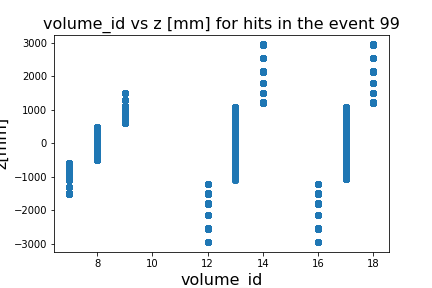
\includegraphics[width=0.35\textwidth]{plots/DataExploration_volume_id_z.png}\\
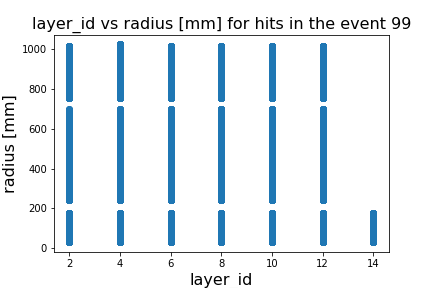
\includegraphics[width=0.35\textwidth]{plots/DataExploration_layer_id_r.png}
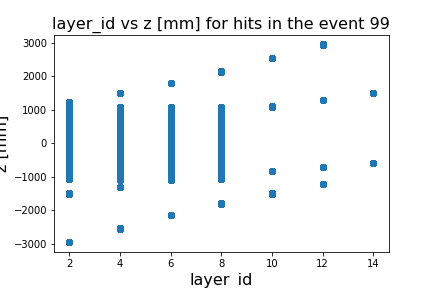
\includegraphics[width=0.35\textwidth]{plots/DataExploration_layer_id_z.png}
\caption{2D scatter plots of the reconstructed hits between the volume ID, module ID versus $r$ and $z$ coordinates, for all truth particles in event 99}
\label{fig:ScatterPlotHits}
\end{figure}

%\ \\ The distribution for one event of the \volumeID~and the \moduleID~inside the detector is illustrated in Figure~\ref{fig:ScatterRZ}.
%
%\begin{figure}[!htb]
%\centering
%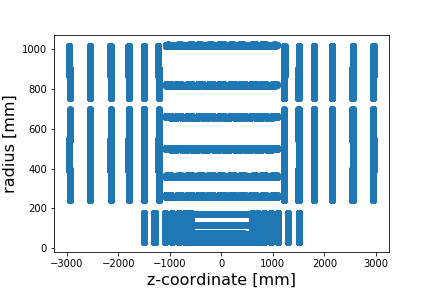
\includegraphics[width=0.7\textwidth]{plots/DataExploration_z_vs_r_scatter.png}
%\caption{2D scatter plots of the reconstructed hits between the $r$ and $z$, for all truth particles in event 99.}
%\label{fig:ScatterRZ}
%\end{figure}



